\section{Virtual Analog Synthesis}

Virtual analog synthesis is the term used to describe the emulation of analog synthsizers of the 60s and 70s digitally in real time. The complexity and goals of an emulation can vary. Some emulations go so far as to simulate the actual electronic components of vintage synthesis circuits, others just model ths signal flow loosly.

Regardless of the type of emulation, and model of analog systhesis has two primary concerns. Latency and aliasing. The problem of latency has already been described above. Any processing will introduce a delay in the signal, the complexity of the processing can increase the delay, or use more CPU cycles. Aliasing is audible distortion introduced by signals that have a higher frequency content than the sampling rate of the system allows for\cite{virtual_analog_synthesis}.

Analog synthsizers usually employed what is refered to as subtractive synthsis. One or more sound generators or oscillators would create signals with particular harmonic qualities. These signals would then go through filters that would "subtract" frequencies from the signal. The oscillators and filters can be modulated as well as the amplitude of the filtered signal. Figure~\ref{fig:synth_voice_block} is a simple block diagram of a typical subtractive synth voice.

\begin{figure}[h]
    \centering
    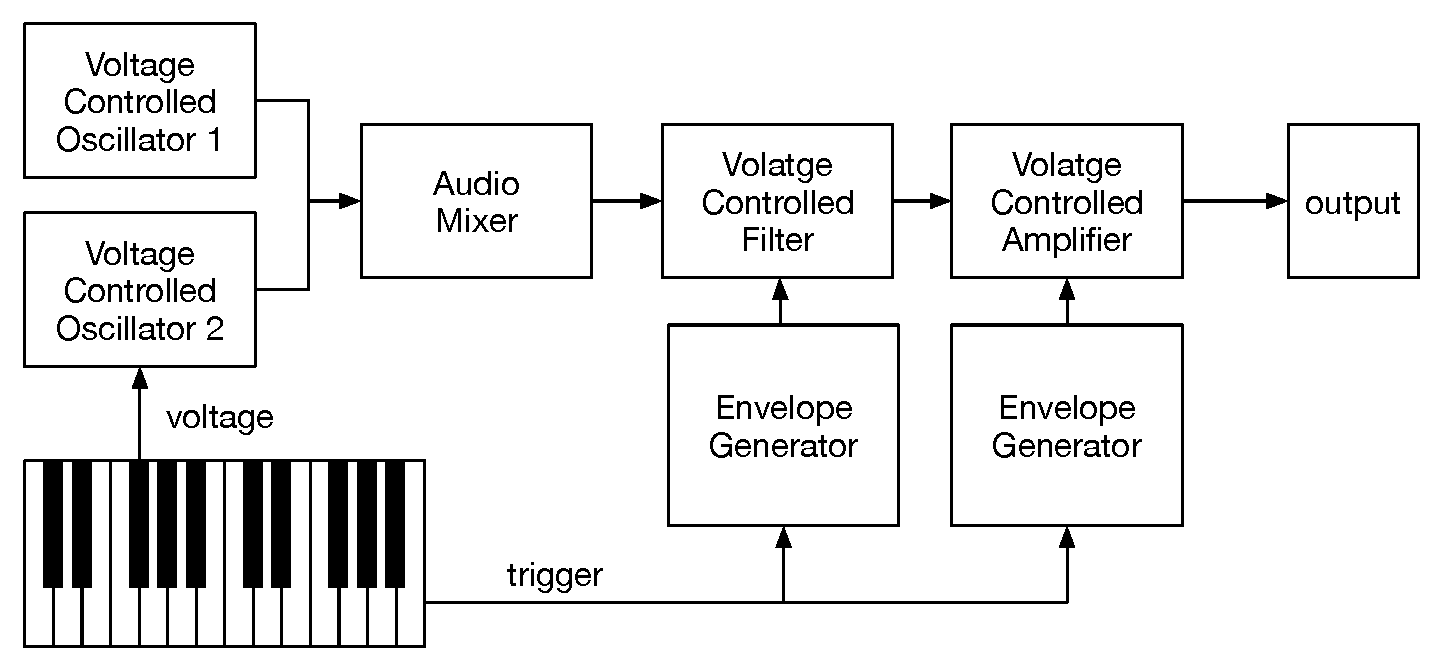
\includegraphics[width=\textwidth]{assets/synth_voice_block.pdf}
    \caption{Block Diagram of a Subtractive Synthesis Voice}
    \label{fig:synth_voice_block}
\end{figure}

The voltage controlled oscillators generate simple waveforms at the pitch coresponding to the note played on the keyboard. The user can typically choose between some combination of sawtooth, squareware, or triangle waveforms. The frequencies or timbre of the waveforms can then be modulated by the following filter and amplitude blocks.

One's first impression might be that modeling the oscillator would be simple. A digitally generated squarewave or sawtooth waveform should be trivial to implement. The 5kHz sawtooch waveform for example, would have a period of 8.82 samples when generated in a 44.1kHz audio environment. So the waveform would increase linearly from -1.0 to 1.0 over a length of 8.82 samples, then jump back to -1.0 and cycle through again. What does 0.82 sample mean in a discreet digital system? Figure~\ref{fig:aliasing_sawtooth} illustrates the problem with a trivial implementation. The left column shows a portion of an idealized 5kHz sawtooth waveform and the coresponding frequency content. Above the 5kHz fundamental frequency are harmonics that will be audible well beyond 100kHz. The right column shows the same portion of a 5khz sawtooth waveform in a 44.1kHz environment. The waveform itself is distorted and the higher harmonics are visible reflected back from the 22.05kHz nyquist limit.

\begin{figure}[h]
    \centering
    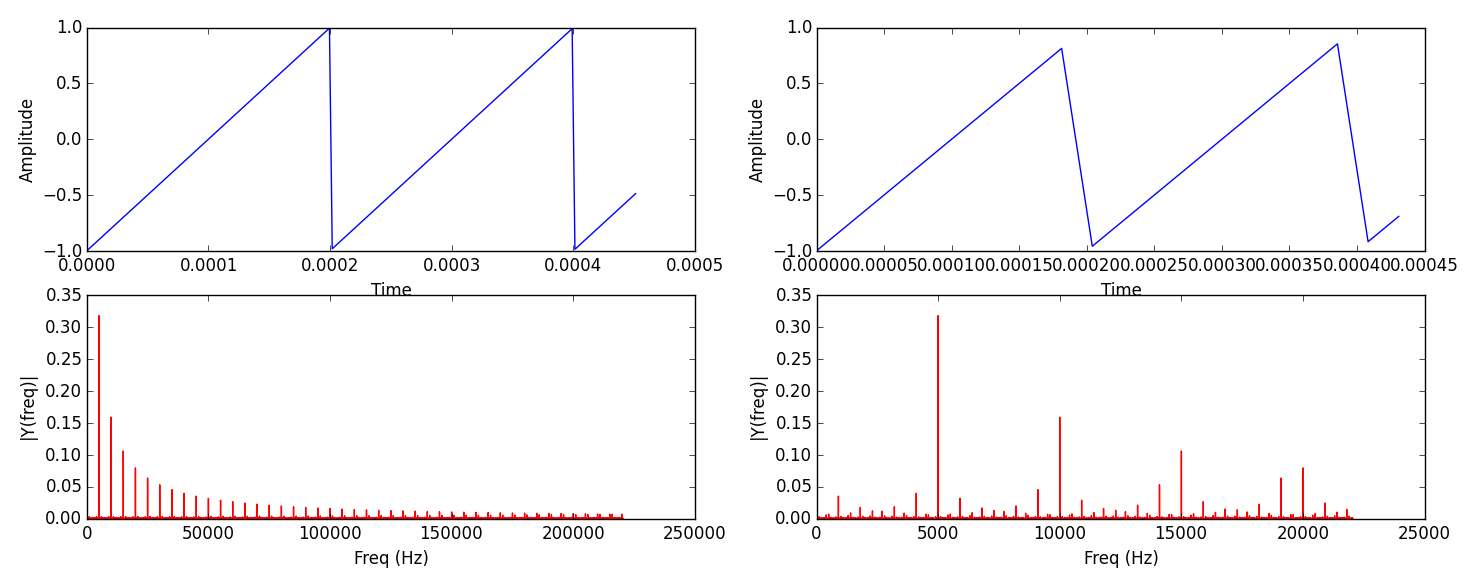
\includegraphics[width=\textwidth]{plots/graphics/sawtooth.png}
    \caption{Ideal and Aliased 5kHz Sawtooth waveform}
    \label{fig:aliasing_sawtooth}
\end{figure}
